\documentclass{beamer}
\usepackage[utf8]{inputenc}
\usepackage[T1]{fontenc}
\usepackage{graphicx}
\usepackage{appendixnumberbeamer}
\usepackage{booktabs}
\usepackage{bbm}
\usepackage[scale=2]{ccicons}
\usepackage{pgfplots}
\usepgfplotslibrary{dateplot}
\usepackage{xspace}
\newcommand{\themename}{\textbf{\textsc{metropolis}}\xspace}

\usetheme{metropolis}

\title{Probability of Successful Transmission of Uplink Messages in LoRaWAN}
%\subtitle{}
\date{\today}
\author{Ante Lojić Kapetanović}
\institute{Department of Electronic Systems @AAU}

\begin{document}

  \maketitle

  \begin{frame}{Content}
    \setbeamertemplate{section in toc}[sections numbered]
    \tableofcontents[hideallsubsections]
  \end{frame}

  \section{Introduction}
  \begin{frame}[fragile]{LoRaWAN}
    \alert{Long Range Wide Area Network} - low power, wide area media access protocol built on top of LoRa designed to wirelesslly connect \textit{things} to the Internet.

    Perfect fit for network of IoT devices that:
    \begin{itemize}
      \item are not power hungry
      \item require minimum bandwidth
      \item send data not to often
    \end{itemize}
  \end{frame}
  \begin{frame}[fragile]
    \begin{center}
      \begin{figure}
        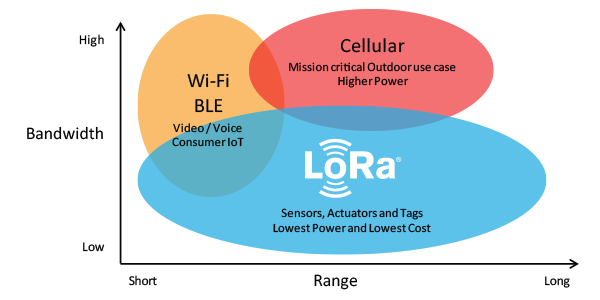
\includegraphics[width=\linewidth]{images/bw_range.png}
      \end{figure}
    \end{center}
  \end{frame}

  \begin{frame}{Infrastructure overview}
    \begin{figure}
      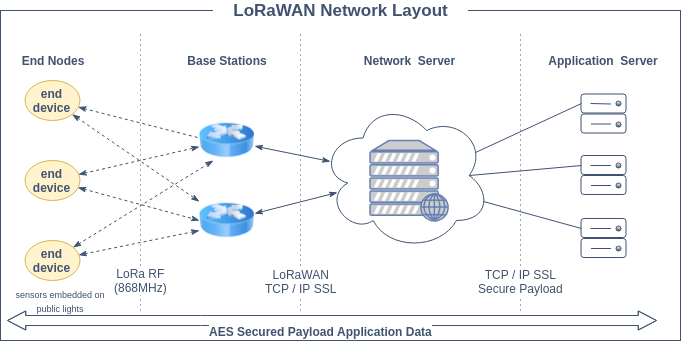
\includegraphics[width=\linewidth]{images/LoRaWAN-Network-Layout.png}
    \end{figure}
  \end{frame}

  \begin{frame}{Svebølle topology}
    \begin{figure}
      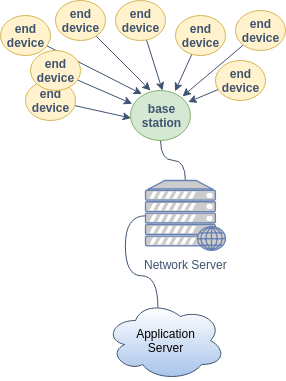
\includegraphics[width=0.48\linewidth]{images/Svebolle-Topology.png}
    \end{figure}
  \end{frame}

  \begin{frame}{Communication model for Svebølle deployment}
    \begin{figure}
      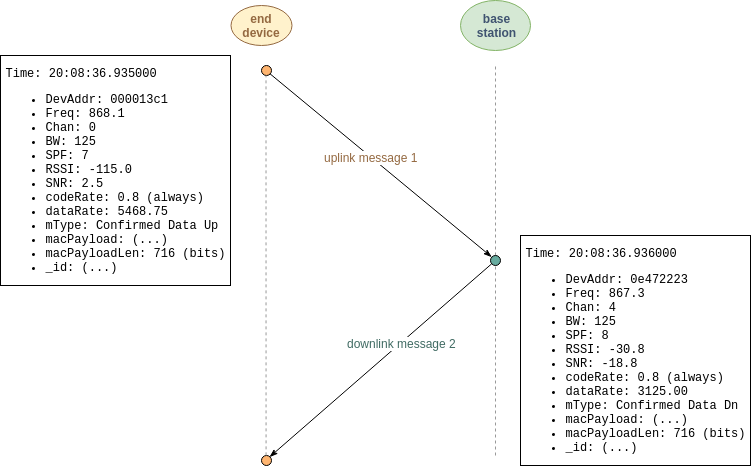
\includegraphics[width=\linewidth]{images/Svebolle-ed-bs-model.png}
    \end{figure}
  \end{frame}

  \begin{frame}{Project goal}
    Is to apply forecasting methods on measured data from the single base station in Svebølle and examine whether there is a possibility of predicting \alert{successful transmission of LoRa messages for given future time interval}.
  \end{frame}

  \section{Predicting future events}
  \begin{frame}{Structure of the measurement data}
    \begin{itemize}
      \item Data was collected during the period of nearly 5 months
      \item 689k measurements are captured on a single base station
      \item Measured features\begin{itemize}
        \item Time
        \item DevAddr
        \item Freq, Chan, BW, CR, DR 
        \item RSSI, SNR  
        \item crcStatus, mType,macPayload 
      \end{itemize}
    \end{itemize}
  \end{frame}

  \begin{frame}{Transformation to time-series}
    \alert{Time-series} data is a series of data points indexed in time order and taken at successive equally spaced points in time.

    To create time series data from given data set, the only important label is wheter the end device has successfully transmitted the message or not. For each time point, where every time point is observation in seconds there is activity flag assigned:
    \begin{itemize}
      \item 1 - device was active for observed time point
      \item 0 - device was not active for observed time point
    \end{itemize}
  \end{frame}

  \begin{frame}{Prediction models}
    \begin{itemize}
      \item Moving average / weighted moving average
      \item Autoregressive integrated moving average (ARIMA)
      \item Holt's winter method
      \item Vector auto regression (VAR)
      \item \alert{Recurrent neural network (RNN)}
      \item Reinforcement learning (RL)
    \end{itemize}
  \end{frame}

  \section{Proposed RNN model}
  \begin{frame}{Artifical neural network}
    Recognizing regularities and patterns of the given data, learning from past experience and providing inference on the output.

    Vanilla ANNs are not perfectly suitable for time-series forecasting because they lack persistance.
  \end{frame}

  \begin{frame}{Reccurent neural network}
    \begin{columns}
      \column{.5\textwidth}
        RNNs contain loops (feedbacks) allowing information to persist.
      \column{.5\textwidth}
      \begin{figure}[]
        \centering
        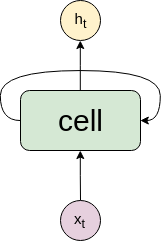
\includegraphics[width=0.6\linewidth]{images/RNN.png}
      \end{figure}
    \end{columns}
  \end{frame}
  \begin{frame}{Unpacked RNN}
    \begin{figure}[]
      \centering
      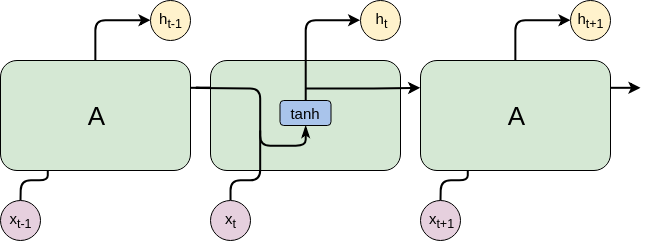
\includegraphics[width=\linewidth]{images/RNN-unpacked.png}
    \end{figure}
  \end{frame}
  \begin{frame}{Short-term memory problem}
    If a sequence is long enough, RNN will have a hard time carrying information from earlier time steps to later ones.
    The reason is that during back propagation, RNNs suffer from the vanishing gradient problem (gradient shrinks during back propagation time).
    \begin{center}
      \textbf{new weight = weight - learning rate * gradient}

      gradient = 0 $\rightarrow$ new weight = weight $\rightarrow$ RNN stops learning 
    \end{center}
  \end{frame}

  \begin{frame}{LSTM networks to the rescue}
    Changing the inner structure of a cell made possible that the flow of information is regulated.

    Inside each LSTM cells there are mechanisms called \alert{gates} that can learn which data in a sequence is important to keep or throw away.
  \end{frame}
  \begin{frame}
    \begin{figure}[]
      \centering
      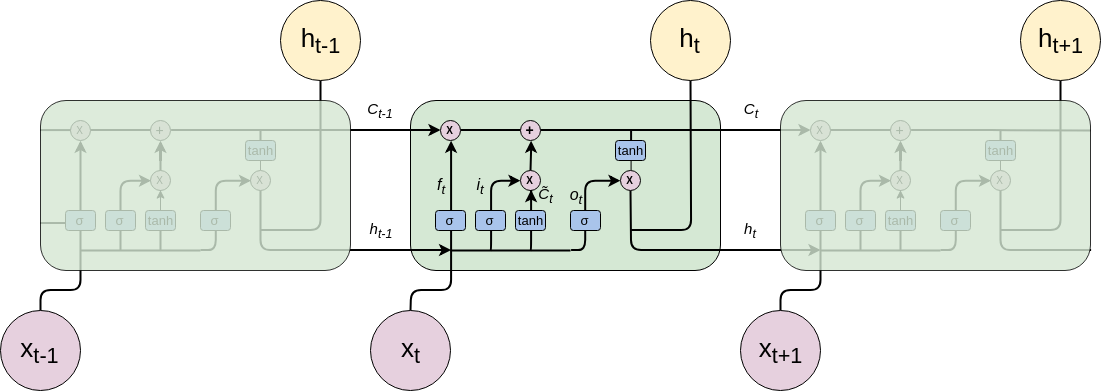
\includegraphics[width=\linewidth]{images/LSTM.png}
    \end{figure}
  \end{frame}

  \begin{frame}{Forget gate}  
    Determines which information to remove from the cell state using sigmoid function that outputs value between 0 (completely reject) and 1 (completely accept)
		$$ f_{t} = \sigma (W_{f} \cdot [h_{t-1}, x_{t}] + b_{f}) $$
		where
		\begin{itemize}
			\item[] $ x_{t} $ is current input vector,
			\item[] $ h_{t-1} $ is previous cell's output value,
			\item[] $ W_{f} $ is associated weight,
			\item[] $ b_{f} $ is added bias.
    \end{itemize}
  \end{frame}

  \begin{frame}{Input gate}
    Decides what new information should be written to the cell state. 
    
    Firstly, the sigmoid function decides which value to update:
    $$ i_{t} = \sigma (W_{i} \cdot [h_{t-1}, x_{t}] + b_{i}) $$ 
    where
    \begin{itemize}
      \item[] $ x_{t} $ is current input vector,
      \item[] $ h_{t-1} $ is previous cell's output value,
      \item[] $ W_{i} $ is associated weight,
      \item[] $ b_{i} $ is added bias.
    \end{itemize}
  \end{frame}

  \begin{frame}{Cell state}
    ...after that, \textit{tanh} layer creates vector of candidates for the cell state:
    $$ \tilde{C}_{t} = tanh (W_{C} \cdot [h_{t-1}, x_{t}] + b_{C}) $$
    where
    \begin{itemize}
      \item[] $ x_{t} $ is current input vector,
      \item[] $ h_{t-1} $ is previous cell's output value,
      \item[] $ W_{C} $ is associated weight,
      \item[] $ b_{C} $ is added bias.
    \end{itemize}
  \end{frame}

  \begin{frame}{Output gate}
    Decides what is going to be output of the concrete cell. 
    $$ o_{t} = \sigma (W_{o} [h_{t-1}, x_{t}] + b_{o}) $$ 
    where
    \begin{itemize}
      \item[] $ x_{t} $ is current input vector,
      \item[] $ h_{t-1} $ is previous cell's output value,
      \item[] $ W_{o} $ is associated weight,
      \item[] $ b_{o} $ is added bias.
    \end{itemize}
    
    The output is based on the filtered version of the cell state.
    $$ h_{t} = o_{t} * tanh(C_{t})$$
    where 
    $ C_{t} $ is the new cell state calclulated as:
    $ C_{t} = f_{t} * C_{t-1} + i_{t} * \tilde{C}_{t} $
  \end{frame}

  \section{Model configuration}
  \begin{frame}{Configuration}
    \begin{itemize}
      \item loss: MSE 
      \item optimizer: ADAM
      \item layers: 3 LSTM (CuDNN implementation)
      \item droput layer with rate of 0.2 after each LSTM layer
      \item batch normalization layer after first two dropouts
      \item last dense layer with only 1 layer has ReLu activation
    \end{itemize}
  \end{frame}

  \section{Probability of device activation for future time period}
  \begin{frame}{Preprocessing}
    \begin{enumerate}
      \item cleansing
      \item clean structured data $\rightarrow$ time-series data
      \item creating sequences
      \item randomizing sequnces  
      \item train-validation split
    \end{enumerate}
  \end{frame}

  \begin{frame}[fragile]{Training}
    In-memory training:
    \begin{itemize}
      \item 10 epochs
      \item 64 batch size
    \end{itemize}
    using 
    \begin{verbatim}
callbacks = [
    EarlyStopping(...),
    ModelCheckpoint(...),
    TensorBoard(...)
    ]  
    \end{verbatim}
  \end{frame}

  \begin{frame}{Validation results}
    \begin{figure}[]
      \centering
      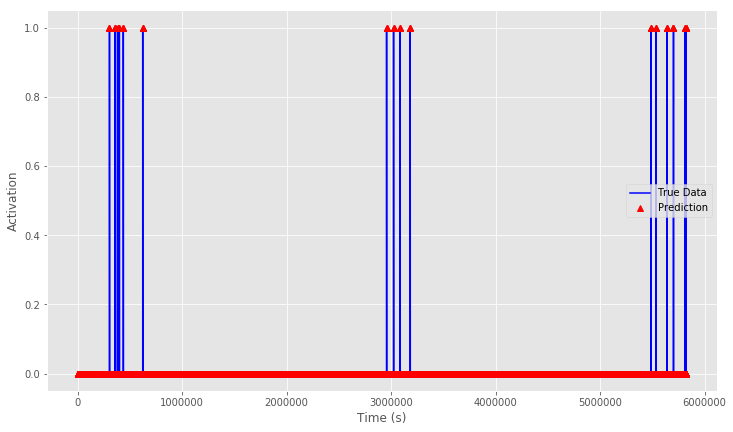
\includegraphics[width=\linewidth]{images/lstm-out.png}
    \end{figure}
  \end{frame}

  \begin{frame}{Probability of successful transmission}
    For given period of time (\textbf{n} seconds) probability of successful transimission of LoRa uplink message should rise up as time period gets bigger (\textbf{n} gets bigger). 
    $$ n = 0 \Rightarrow p_{st} = 0 $$ 
    $$ n \in <0, +\infty> \Rightarrow p_{st} \in <0, 1> $$
    $$ n = \infty \Rightarrow p_{st} = 1 $$

    Probability can be calclulated as: 
    $$ \mathbb{P}[N_{t} = k | X] =  \frac{1}{s-t}  \sum_{i=0}^{s-t}\mathbbm{1}[\sum_{j=0}^{t}X[i+j]=k] $$
  \end{frame}

  \begin{frame}
    \begin{figure}[]
      \centering
      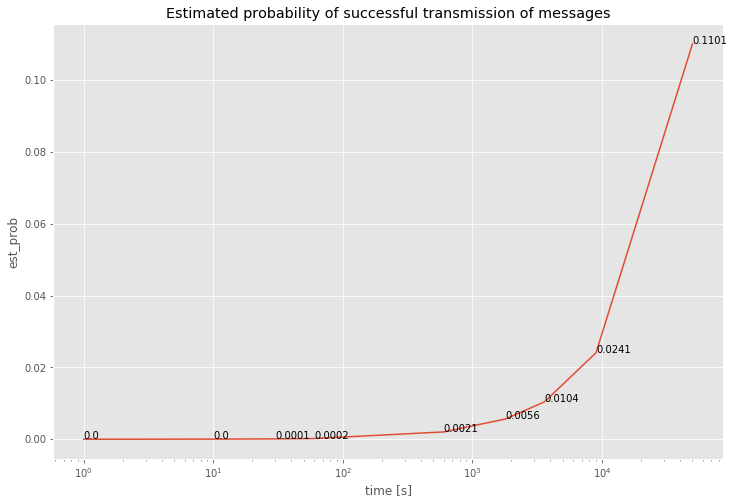
\includegraphics[width=\linewidth]{images/est-prob.png}
    \end{figure}
  \end{frame}


  \section{Conclusion}
  \begin{frame}{Future work}
    \begin{itemize}
      \item \textbf{Multivariate time-series data} instead of univariate time-series data: observe not only previous historical events for specific device but also activation of other devices
      \item \textbf{Longer training sequences}
      \item Future \textbf{sequence predictions} instead of point-to-point predictions
    \end{itemize}
  \end{frame}

  \begin{frame}[standout]
    Questions?
  \end{frame}

  
\end{document}